In diesem Abschnitt soll auf die Datenaufnahme, sowie alle nötigen Schritte der Datenverarbeitung bis zur fertigen $g^{(2)}(\tau)$-Funktion eingegangen werden. 
Dafür werden zuerst die Datenaufnahme und dafür nötige Kalibrationsverfahren erläutert. 
In diesem Zuge wird zudem auf das Aussehen der aufgenommenen Daten (Waveforms) eingegangen. 
Anschließend werden korrelierte Einzeldateien betrachtet und es wird verdeutlicht, warum eine Mittelung vieler Waveforms unumgäglich ist. 
Zuletzt werden angewandte Korrekturen und Filter angesprochen, sowie verdeutlicht, wie die Mittelung der Daten erfolgt. 

\subsection{Datenaufnahme und Waveforms}
\label{ssec:Datenaufnahme und Waveforms}
Die Aufnahme der Daten erfolgt durch ein von der Arbeitsgruppe geschriebenes Programm, welches mit den ADCs kommuniziert. Ein Screenshot der GUI, worauf die wichtigsten Schritte der Datenaufnahme markiert sind, ist in \autoref{fig:Screenshot GUI} eingefügt. 
\begin{figure}[htbp]
    \centering
    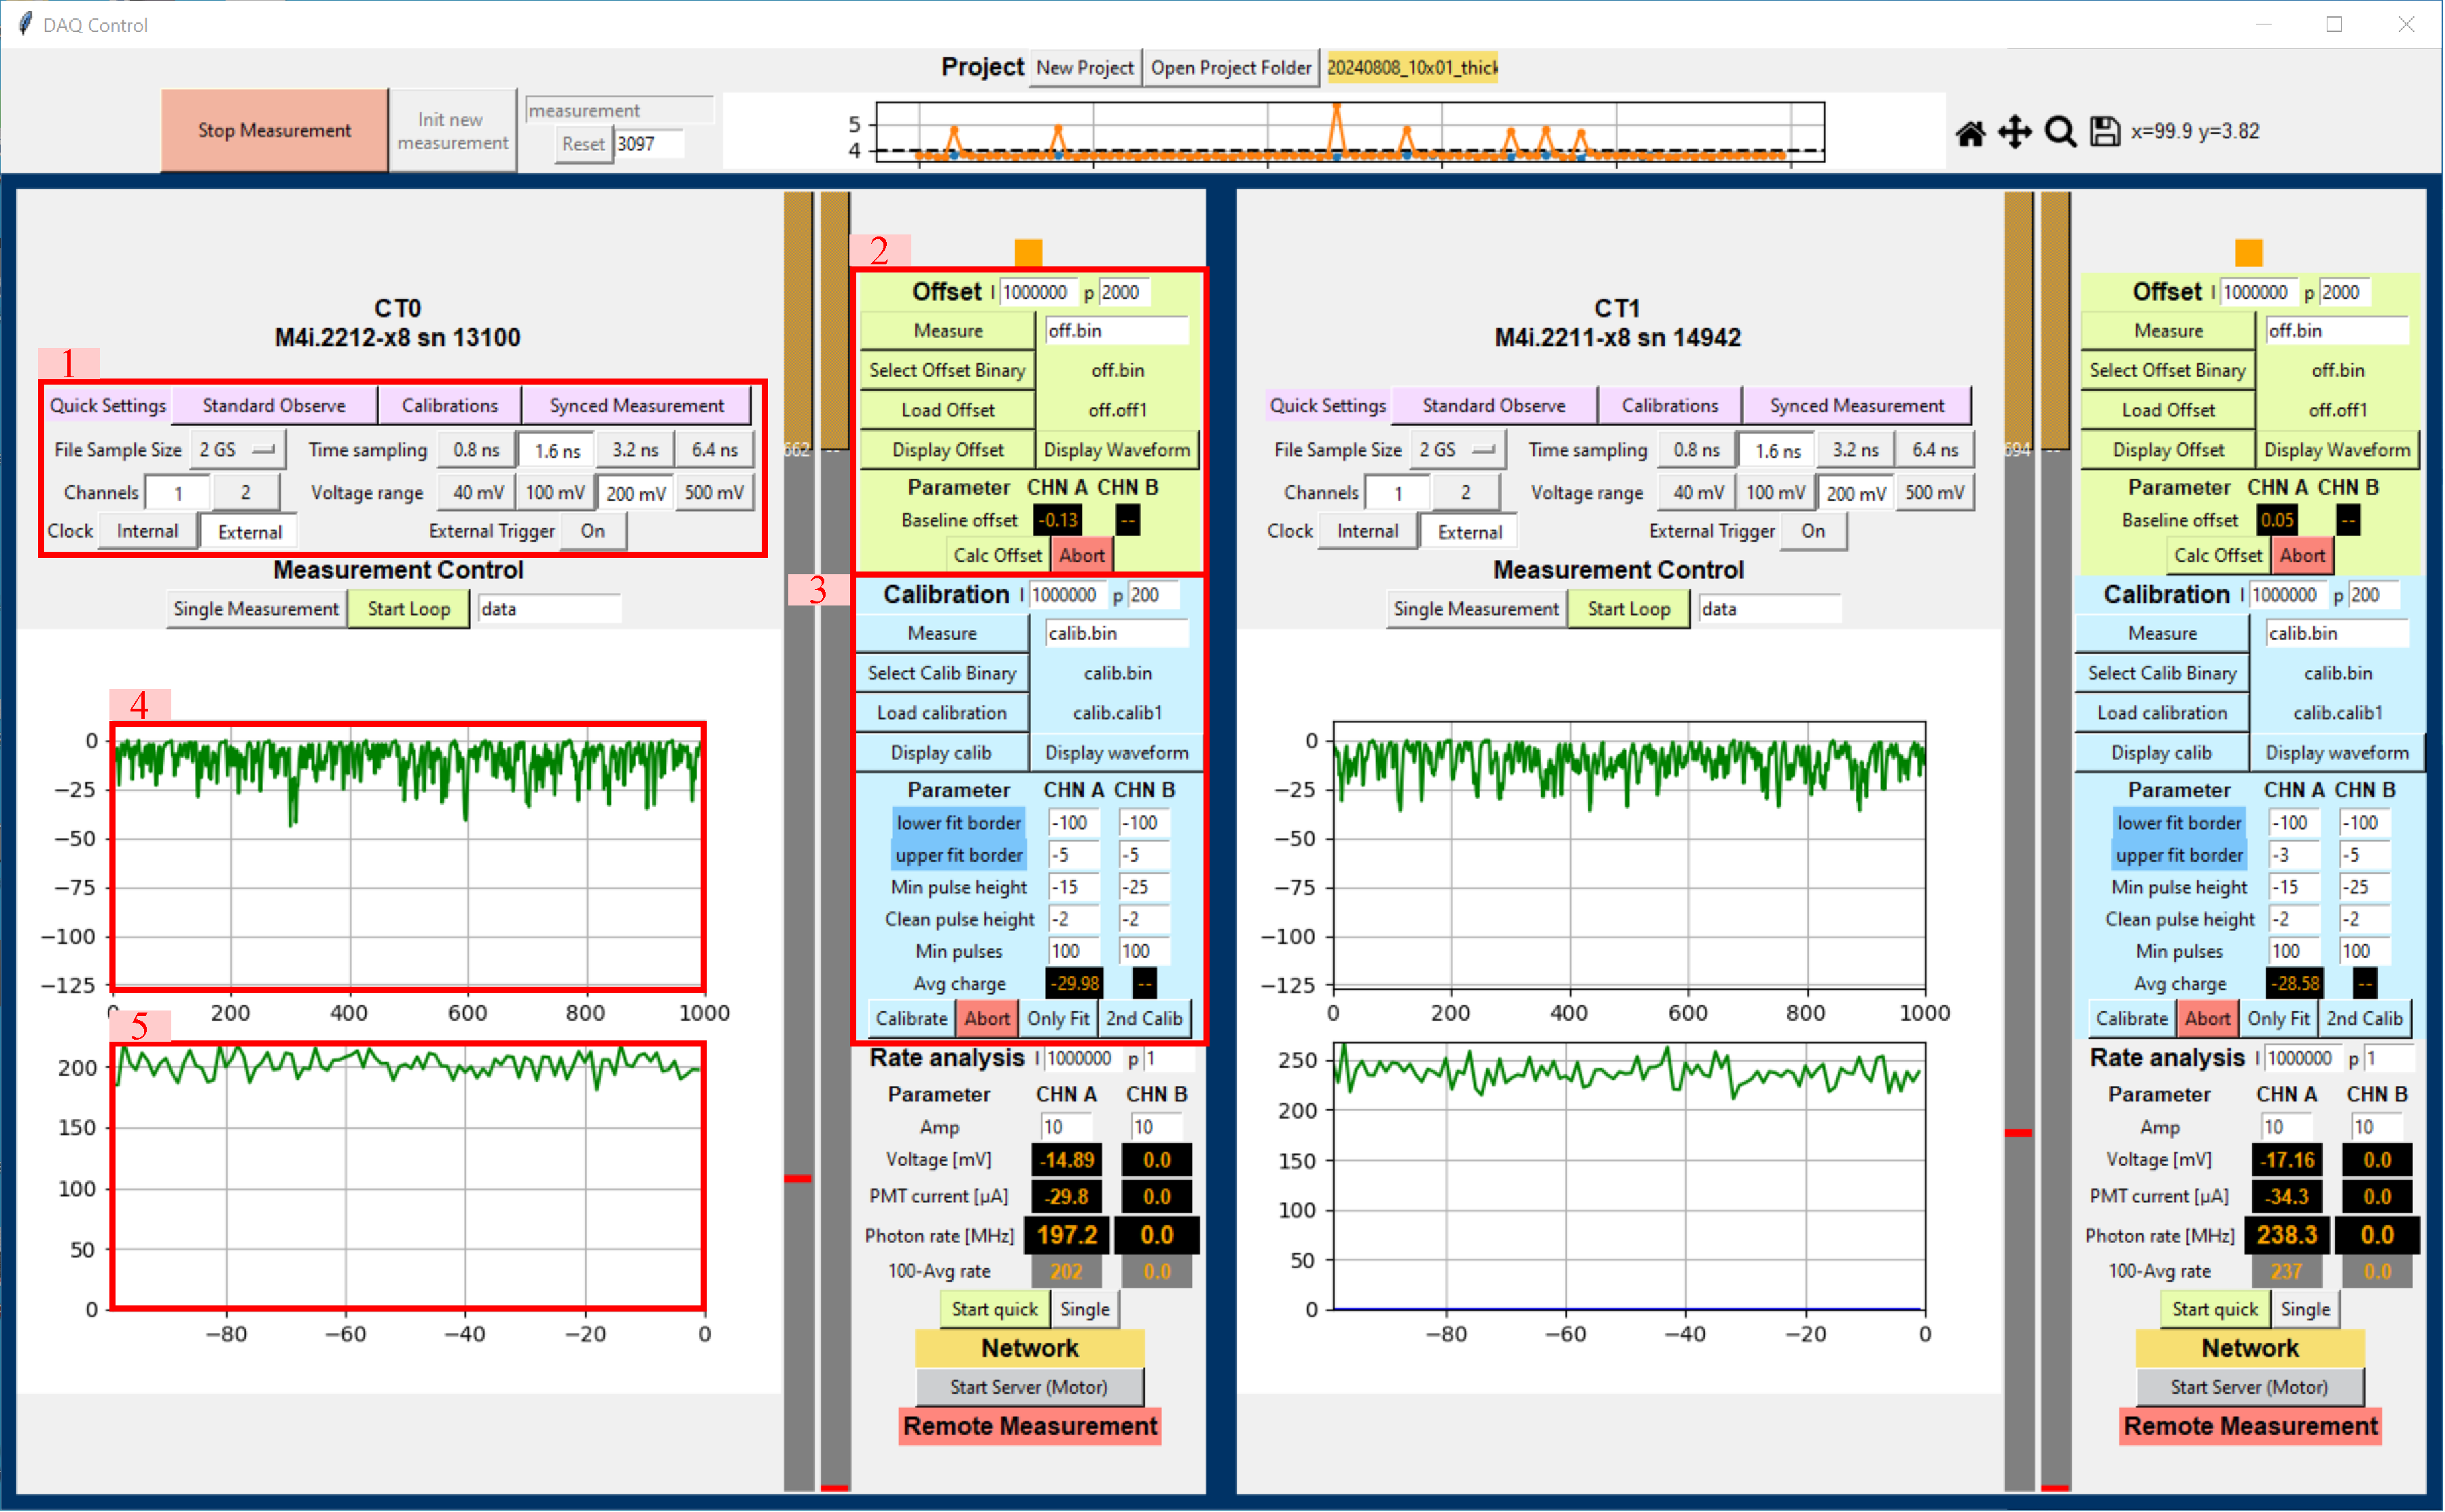
\includegraphics[width=0.9\textwidth]{images/Datenaufnahme/GUI.pdf}
    \caption{Dargestellt ist ein Screenshot der GUI zur Datenaufnahme. Wichtige Schritte sind markiert.}
    \label{fig:Screenshot GUI}
\end{figure}
In der GUI wird für jede verwendete Digitalisierungskarte ein Fenster erstellt, indem Einstellungen für die jeweilige Karte vorgenommen werden können. 
Nach dem Erstellen eines Projekts können in dem mit \emph{1} markierten Bereich in \autoref{fig:Screenshot GUI} Einstellungen für die ADC-Karte vorgenommen werden. 
Es wird mit einem Kanal je Karte gemessen, die Samplingzeit beträgt 1,6\,ns bei einer Dateigröße von 2 Gigasamplen. 
Der zu digitalisierende Spannungsbereich wird passend zu den in \emph{4} abgebildeten Waveforms auf 200\,mV gesetzt. 
Clock und Trigger werden extern durch das White Rabbit System gegeben. 
Die genannten Einstellung werden größtenteils vor der Messung automatisch mit dem Button \glqq Init new measurement\grqq\;gesetzt. \\
Vor Start der Messung müssen zwei Kalibrationsschritte für jeden Kanal gemacht werden. 
Zuerst wird unter \emph{2} eine Offset Kalibration durchgeführt, indem \glqq Measure\grqq\; und \glqq Calc Offset\grqq\; gewählt wird. 
Diese wird ohne Beleuchtung und mit ausgeschaltener Hochspannung durchgeführt. 
Das Programm bestimmt diesen vom PMT abhängigen Offset und entfernt diesen, sodass dieser die Korrelation nicht beeinflusst \cite{zmijaOpticalIntensityInterferometry2021}. 
Anschließend wird bei eingeschaltener Hochspannung und niedriger Photonenrate eine Raten-Kalibration durchgeführt, sodass gemessene Spannungen in Photonenraten umgerechnet werden können. 
Dies ist nötig, da aufgrund der hohen Raten bei der Messung nicht Einzelphotonepulse, sondern ganze Waveforms miteinander korreiert werden. 
Für die Kalibration werden für jeden Kanal die mittlere Pulsform der PMT-Pulse bestimmt und gespeichert. 
Es wird erwartet, dass diese einen bedeutenden Einfluss auf die Form der $g^{(2)}$-Funktion hat, da die Pulse deutlich breiter sind als die einzelnen 1,6\,ns-Bins \cite{zmijaOpticalIntensityInterferometry2021}. 
Aus den gemessenen Daten wird bestimmt wie viel Ladung ein Photon das auf einen PMT trifft durchschnittlich freisetzt, woraus anschließend die in \emph{5} gezeigten Photonenraten in MHz bestimmt werden können. \\
Nach diesen Kalibrationsschritten kann die Messung gestartet werden, woraufhin alle 4\,s 2$\cross$2\,GS an Daten aufgenommen werden. 
Da jedes Sample einem 8\,bit ADC-Wert entspricht, erreicht die MEssung also eine Datenrate von 2$\cross$2\,GB, was erklärt, weshalb die Daten erst gespeichert und anschließend offline korreliert werden.  
Zur Veranschaulichung ist in \autoref{label} aufgezeigt, wie eine typische Waveform zur Offset-, bzw. Raten-Kalibration und zur Messung aussieht. 
\todo{figure}



\subsection{Korrelation}
\label{ssec:Korrelation}
Die Korrelation der Daten erfolgt parallelisiert nachdem die Datenaufnahme abgeschlossen ist. 
Jede Datei von beiden Kanälen wird getrennt miteinander korreliert, indem diese zuerst in Vektoren $\mathbf{A}$ und $\mathbf{B}$ eingelesen werden. 
Anschließend wird für jede Zeitdifferenz $\tau$ das folgende Skalarprodukt berechnet: 
\begin{equation}
    G^{(2)}(\tau) = \mathbf{A}(t)\cdot\mathbf{B}(t+\tau)
\end{equation}
Damit entspricht jeder Wert von $G^{(2)}(\tau)$ der unnormalisierten zeitlichen Photonenkorrelation zu diesem Zeitpunkt \cite{zmijaOpticalIntensityInterferometry2021}. 
Die korrelierten Einzeldateien können anschließend für die weitere Datenanalyse gespeichert werden, da diese deutlich kleiner (im Bereich ieniger kB) sind als die Rohdaten. 
Um aus der bestimmten $G^{(2)}$-Funktion die normierte zeitliche Korrelationsfunktion zu erhalten, wird diese durch ihren Mittelwert weit außerhalb des Bunching Peaks geteilt:
\begin{equation}
    g^{(2)}(\tau) = \frac{G^{(2)}(\tau)}{\overline{G^{(2)}(\tau\gg\tau_c)}}
\end{equation}
Ein Beispiel für die unnormierte Funktion $G^{(2)}$ einer einzelnen Datei ist in \autoref{label} dargestellt. 
\begin{figure}[htbp]
    \centering
    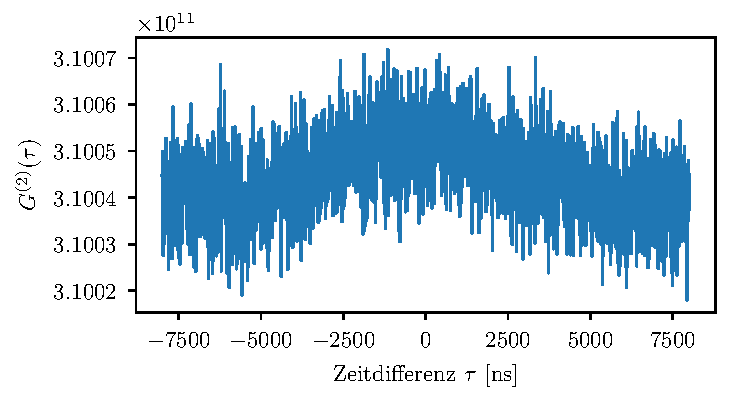
\includegraphics{images/Datenaufnahme/G2.pdf}
    \caption{Ein Beispiel einer unnormierten Korrelationsfunktion ist abgebildet. Durch das verrauschte Signal ist an der Stelle $\tau=0$ kein Bunching Peak sichtbar.}
    \label{fig:G2(tau)}
\end{figure}
Es ist ersichtlich, dass die Funktion stark verrauscht ist und der Bunching Peak nicht auszumachen ist. 
Die in \autoref{ssec:Intensitäteninterferometrie} bereits erwähnte Nowendigkeit der Mittelung über viele Daten, d.h. lange Zeiten um die Form von $g^{(2)}$ bestimmen zu können ist daher deutlich sichtbar. 

\todo{...}
\begin{figure}[htbp]
    \centering
    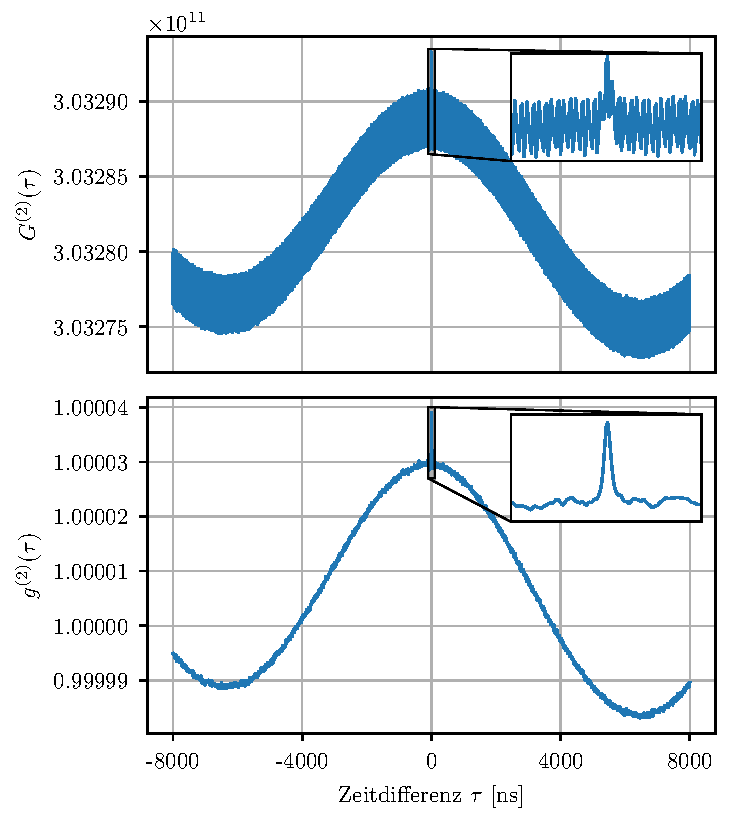
\includegraphics{images/Datenaufnahme/G2_vs_g2.pdf}
    \caption{<caption>}
    \label{<label>}
\end{figure}